\documentclass[12pt,a4paper]{ctexart}
\usepackage[margin=2.5cm]{geometry}
\usepackage{graphicx}
\usepackage{enumitem}
\usepackage{longtable}
\usepackage{array}
\usepackage{booktabs}
\usepackage{xcolor}
\usepackage{tabularx}
\usepackage{titlesec}
\usepackage{float}
\usepackage{hyperref}
\hypersetup{colorlinks=true,linkcolor=blue,urlcolor=blue}

\titleformat{\section}{\Large\bfseries}{\thesection}{1em}{}
\titleformat{\subsection}{\large\bfseries}{\thesubsection}{1em}{}

\graphicspath{{img/}}

\title{\textbf{Offer Show 微信公众号后台系统\\ 文档二：需求文档}}
\author{顾远\quad 23301095}
\date{2026 年 4 月 27 日}

\begin{document}
\maketitle
\tableofcontents
\newpage

\section{文档概述}

\subsection{编写目的}
本文档面向 Offer Show 微信公众号后台系统中“\textbf{找名企 $\rightarrow$ 名企实习校招}”、“\textbf{查薪资 $\rightarrow$ *}”业务模块，
通过对 Offer Show 微信小程序对应页面的调研，整理并形成完整的功能性需求与非功能性需求，
为后续系统详细设计（文档三）以及后台代码实现提供依据。

\subsection{业务范围}
本文档覆盖小程序两大业务模块：
\begin{itemize}[leftmargin=2em]
    \item \textbf{找名企 $\rightarrow$ 名企实习校招}：招聘信息列表（首页 Feed 流）；行业、意向城市、招聘类型多维筛选；招聘详情（招聘信息 / 招聘岗位 / 招聘简介 / 公司简介）；求职早报订阅；求职好课与求职专栏；内推集合、实习点评榜、顶尖人才计划、社招集合。
    \item \textbf{查薪资}：薪资爆料分享（用户提交）；薪资最新动态（Feed 流）；薪资人气榜单（周榜 / 月榜）；校招薪资查询；社招薪资查询。
\end{itemize}

\subsection{术语与缩写}
\begin{tabularx}{\textwidth}{lX}
\toprule
\textbf{术语} & \textbf{说明}\\
\midrule
招聘信息 & 由企业发布的一条完整的招聘机会，包含公司、批次、岗位、城市、链接等\\
招聘批次 & 校招正式批 / 春招正式批 / 春招提前批 / 暑期实习 / 日常实习 / 社会招聘 等\\
内推码 & 投递时使用的专属推荐编码，可提升筛选优先级\\
点评 & 用户对实习企业的评分（0--10 分）与文字评论\\
薪资爆料 & 用户匿名提交的薪资 offer 详情，含公司、岗位、城市、薪资描述、备注等\\
可信度 & 系统结合提交人历史与社区互动给出的薪资爆料可信度评分\\
SP / SSP & Special / Super Special Offer，行业内对高于普通档位 Offer 的称呼\\
\bottomrule
\end{tabularx}

\section{用户与角色}
\begin{longtable}{p{3cm}p{4cm}p{8cm}}
\toprule
\textbf{角色} & \textbf{身份} & \textbf{典型权限}\\
\midrule
\endhead
游客 & 未登录用户 & 浏览部分招聘列表、查看公司简介摘要；不可订阅、不可点评、不可领取内推码\\
普通用户 & 微信授权登录用户 & 全部浏览、筛选、订阅早报、收藏、加入日程、复制投递链接、提交点评\\
会员用户 & 付费开通会员 & 在普通用户基础上享受"最新招聘提前看"、专属内推、求职好课折扣等\\
HR / 企业 & 经审核的企业账号 & 创建/更新/删除本企业的招聘信息、批量上传岗位\\
管理员 & 平台运营 & 审核招聘信息、管理行业/城市字典、封禁作弊用户、批量操作\\
\bottomrule
\end{longtable}

\section{功能性需求（找名企 $\rightarrow$ 名企实习校招）}

\subsection{招聘信息首页}
对应小程序"找名企 $\rightarrow$ 名企实习校招"主页面，参考截图如图~\ref{fig:findco-home} 所示。
\begin{figure}[H]
    \centering
    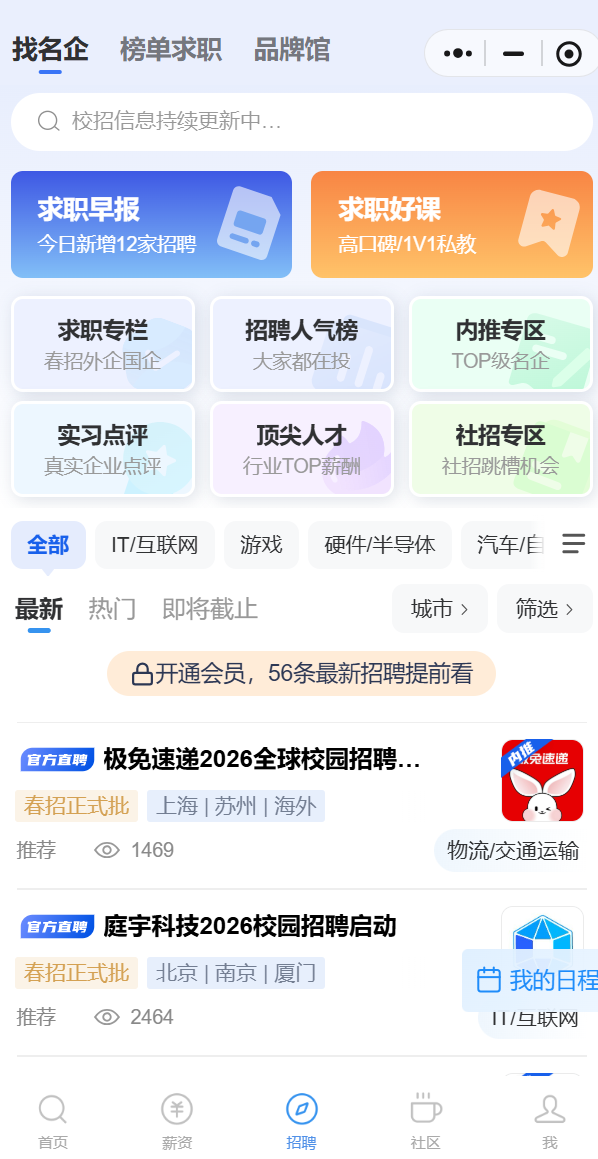
\includegraphics[width=0.32\textwidth]{image-20260427143510279.png}
    \caption{名企实习校招首页（含搜索、九宫格入口、行业 Tab、列表）}
    \label{fig:findco-home}
\end{figure}
\paragraph{功能点}
\begin{enumerate}[leftmargin=2em]
    \item 顶部搜索框：支持关键字（公司名 / 岗位名）实时检索，例如输入"字节跳动"返回相关招聘列表。
    \item 入口卡片九宫格：求职早报、求职好课、求职专栏、招聘人气榜、内推专区、实习点评、顶尖人才、社招专区。
    \item 全局筛选 Tab：行业（全部 / IT 互联网 / 游戏 / 硬件半导体 / 汽车 …）。
    \item 排序 Tab：最新 / 热门 / 即将截止。
    \item 二级筛选：城市、更多筛选（行业+招聘类型组合）。
    \item 列表项展示：公司 LOGO、招聘标题、批次标签、工作城市、浏览数、官方直聘 / 推荐标识、所属行业。
    \item 会员引导横幅：例如"开通会员，56 条最新招聘提前看"。
    \item 分页：支持下拉刷新、上拉加载更多，按页大小（默认 20 条）分页查询。
\end{enumerate}

\subsection{行业筛选}
\paragraph{功能点}
\begin{itemize}[leftmargin=2em]
    \item 单选模式，默认值"全部"。
    \item 行业枚举值（来自字典服务，可由管理员维护）：全部、IT/互联网、游戏、硬件/半导体、汽车/自动驾驶、机械/制造业、金融行业、消费生活、医疗健康、政府/事业单位、国企央企、广告传媒、建筑/房地产、材料/能源/化工、物流/交通运输、其他行业。
    \item 选中后回到列表页并刷新结果。
\end{itemize}

\subsection{意向城市筛选}
\paragraph{功能点}
\begin{itemize}[leftmargin=2em]
    \item 多选模式，默认值"全部"。
    \item 内置热门城市集合：北京、上海、广州、深圳、杭州、成都、武汉、苏州、南京、天津、郑州、合肥、长沙、济南、太原、青岛、石家庄、西安、重庆、厦门、宁波、福州、昆明、南昌、佛山、东莞 等。
    \item 操作按钮：重置、确定。
    \item 与列表页共享筛选状态，二次进入保留上次选择。
\end{itemize}

\subsection{更多筛选}
\paragraph{功能点}
\begin{itemize}[leftmargin=2em]
    \item 所在行业（多选）。
    \item 招聘类型（多选）：不限、校招、实习、日常实习、暑期实习、春招提前批、春招正式批、春招补录、秋招提前批、秋招正式批、秋招补录、校招提前批、校招正式批、校招补录。
    \item 重置 / 确定双按钮，确定后将筛选条件应用到列表 API 请求。
\end{itemize}

\subsection{招聘详情}
点击一条招聘信息进入。共 4 个 Tab：招聘信息、招聘岗位、招聘简介、公司简介，如图~\ref{fig:findco-detail} 所示。
\begin{figure}[H]
    \centering
    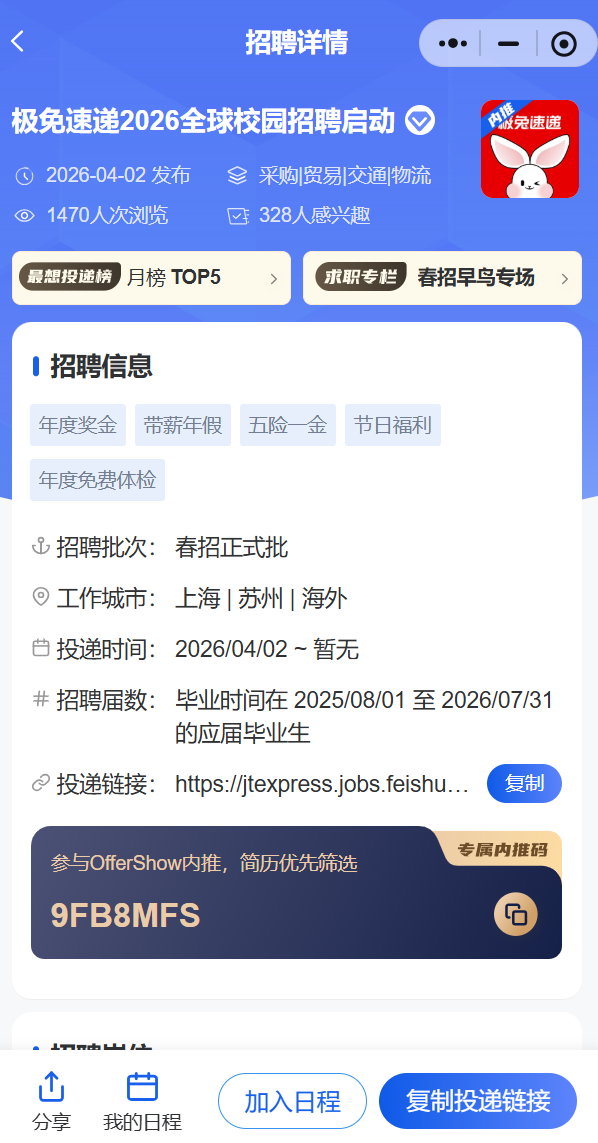
\includegraphics[width=0.30\textwidth]{image-20260427143739496.png}
    \caption{招聘详情页（招聘信息 Tab）}
    \label{fig:findco-detail}
\end{figure}
\paragraph{招聘信息 Tab}
\begin{itemize}[leftmargin=2em]
    \item 头部：公司 LOGO、标题、发布日期、采购/贸易/交通/物流等岗位类别、浏览次数、感兴趣人数、暑期投递榜月榜、求职专栏标签。
    \item 福利标签：年度奖金、带薪年假、五险一金、节日福利、年度免费体检 等。
    \item 详细字段：招聘批次、工作城市、投递时间、招聘届属、投递链接（一键复制）。
    \item OfferShow 内推区：专属内推码（如 9FB8MFS），简历优先筛选。
    \item 底部操作栏：分享、我的日程、加入日程、复制投递链接。
\end{itemize}
\paragraph{招聘岗位 Tab}
列表展示该批次下开放的所有岗位类别，例如"物流营运类、产品研发类、财务审计类、小语种类、综合职能类、海外地区岗、实习生"等。
\paragraph{招聘简介 Tab}
含【招聘对象】、【专属福利】、【招聘流程】、【投递须知】等富文本段落。
\paragraph{公司简介 Tab}
公司 LOGO、公司名、行业地位简述、规模、覆盖国家/地区、企业文化等富文本字段。

\subsection{求职早报}
对应页面如图~\ref{fig:findco-daily} 所示。
\begin{figure}[H]
    \centering
    
\includegraphics[width=0.30\textwidth]{image-20260427143835052.png}
    \caption{求职早报订阅页}
    \label{fig:findco-daily}
\end{figure}
\paragraph{功能点}
\begin{itemize}[leftmargin=2em]
    \item 顶部 Banner，订阅按钮："订阅早报，获取当日最新招聘信息"。
    \item 周历日期切换：按日（周一--周日）查看每日早报。
    \item 加群入口："加入群聊，接收最新招聘推送 $\rightarrow$ 立即进群"。
    \item 24h 新招列表，展示公司、岗位、批次、城市、行业。
    \item 用户可订阅 / 取消订阅，订阅状态写入用户偏好。
\end{itemize}

\subsection{求职好课}
对应页面如图~\ref{fig:findco-course} 所示。
\begin{figure}[H]
    \centering
    
\includegraphics[width=0.30\textwidth]{image-20260427143906716.png}
    \caption{求职好课页面}
    \label{fig:findco-course}
\end{figure}
\paragraph{功能点}
\begin{itemize}[leftmargin=2em]
    \item 课程分类 Tab：全部课程、求职必备、行业好课、求职陪跑。
    \item 课程卡片：封面、标题（如"27/28 届校招求职陪跑"、"1v1 私教 简历精修--校招版/社招版"、"1v1 私教 大厂面试官模拟面试"）、简介、价格（如 \textyen 12980 / 599 / 14980）。
    \item 点击进入课程详情或购买流程（购买流程不在本系统范围内，提供跳转链接）。
\end{itemize}

\subsection{求职专栏}
以"金融科技专场"为例，对应页面如图~\ref{fig:findco-column} 所示。
\begin{figure}[H]
    \centering
    
\includegraphics[width=0.30\textwidth]{image-20260427145341240.png}
    \caption{求职专栏（金融科技专场示例）}
    \label{fig:findco-column}
\end{figure}
\paragraph{功能点}
\begin{itemize}[leftmargin=2em]
    \item 专栏 Tab：金融科技专场、AI 专场、春招补录专场、春招早鸟专场、国企央企优选、互联网优选、寒暑假实习专场、半导体专场、优质外企 等。
    \item 顶部统计：在招企业数、累计浏览人次（如 472 家正在招聘、66325 人次浏览）。
    \item 列表与首页相同的字段、相同的排序与筛选能力。
\end{itemize}

\subsection{内推集合（OfferShow 内推合集）}
对应页面如图~\ref{fig:findco-refer} 所示。
\begin{figure}[H]
    \centering
    
\includegraphics[width=0.30\textwidth]{image-20260427145407886.png}
    \caption{OfferShow 内推合集}
    \label{fig:findco-refer}
\end{figure}
\paragraph{功能点}
\begin{itemize}[leftmargin=2em]
    \item 列表展示带"官方直聘 / 国企 / 外企"等标签的内推机会。
    \item 字段：公司、批次（春招提前批 / 秋招正式批 / 暑期实习 …）、城市、浏览数、行业、状态（尽快投递）。
    \item 点击进入对应招聘详情页。
\end{itemize}

\subsection{实习点评榜}
对应页面如图~\ref{fig:findco-review} 所示。
\begin{figure}[H]
    \centering
    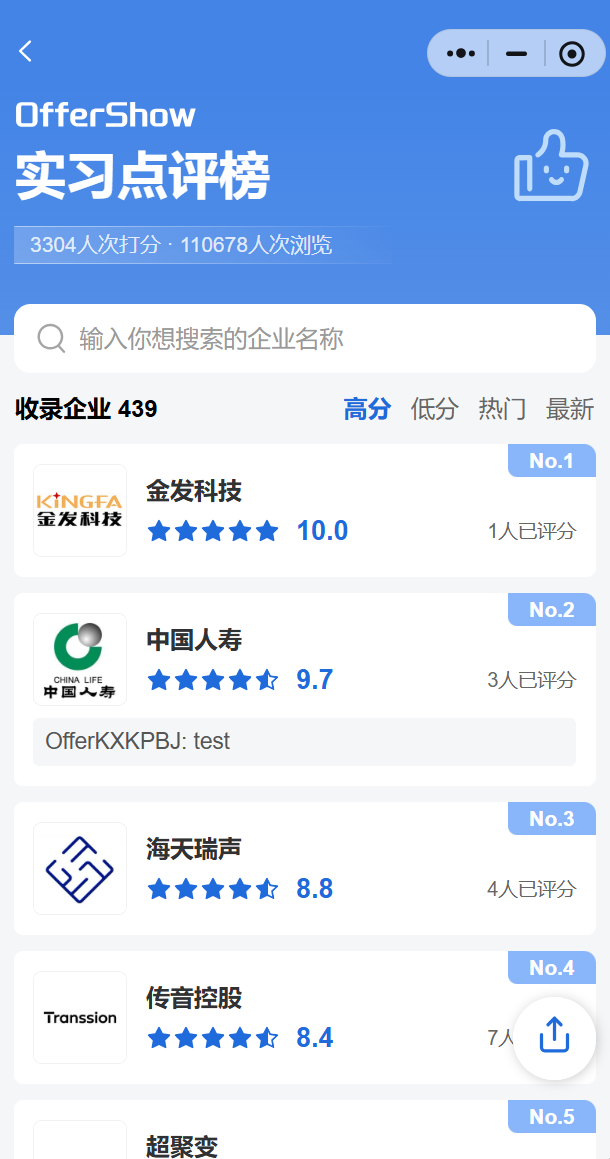
\includegraphics[width=0.30\textwidth]{image-20260427145431365.png}
    \caption{实习点评榜}
    \label{fig:findco-review}
\end{figure}
\paragraph{功能点}
\begin{itemize}[leftmargin=2em]
    \item 顶部 Banner：累计打分人次、浏览人次（如 3304 人次打分 · 110678 人次浏览）。
    \item 搜索框："输入你想搜索的企业名称"，支持模糊检索。
    \item 排行榜 Tab：高分、低分、热门、最新。
    \item 列表项：排名 No.x、企业 LOGO、企业名、星级评分（0--10 分）、已评分人数、最新一条简短点评。
    \item 普通用户可对企业进行打分与评论；管理员可下架不当评论。
\end{itemize}

\subsection{顶尖人才计划}
对应页面如图~\ref{fig:findco-elite} 所示。
\begin{figure}[H]
    \centering
    
\includegraphics[width=0.30\textwidth]{image-20260427145457276.png}
    \caption{顶尖人才计划}
    \label{fig:findco-elite}
\end{figure}
\paragraph{功能点}
\begin{itemize}[leftmargin=2em]
    \item 列表展示各大厂高薪计划，如"阿里星 A Star 顶尖人才计划"、"京东 TGT 顶尖青年技术天才计划"。
    \item 字段：薪资范围（如 100--200 万 / 年）、计划介绍、跳转链接。
    \item 顶部统计：超高薪机会数、高薪数据分享数（27 个超高薪机会、123595 人次浏览）。
\end{itemize}

\subsection{社招集合（OfferShow 社招计划合集）}
对应页面如图~\ref{fig:findco-social} 所示。
\begin{figure}[H]
    \centering
    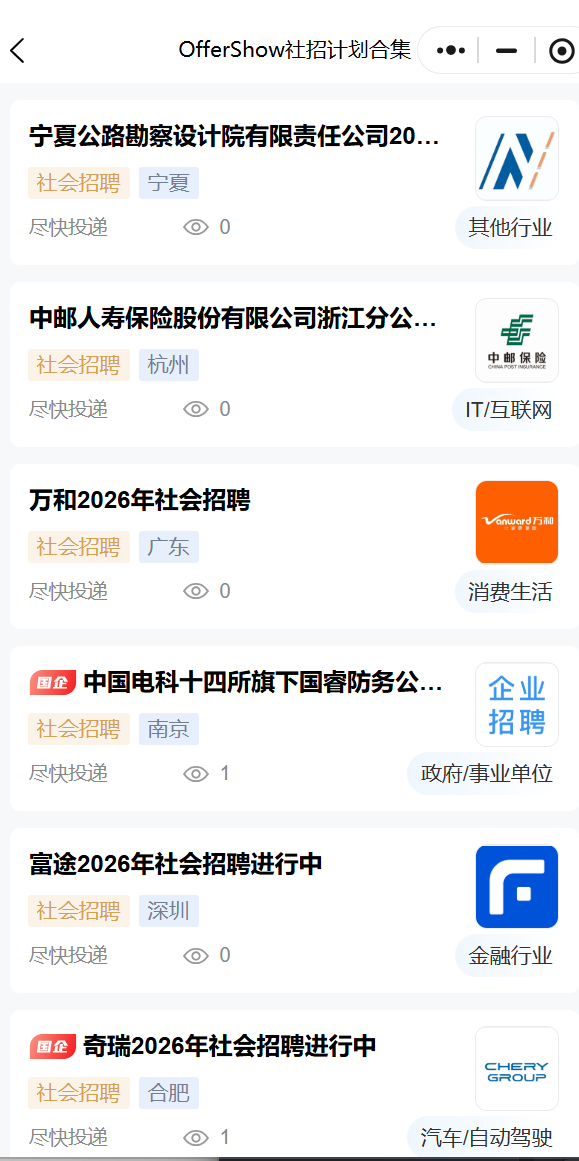
\includegraphics[width=0.30\textwidth]{image-20260427145553499.png}
    \caption{OfferShow 社招计划合集}
    \label{fig:findco-social}
\end{figure}
\paragraph{功能点}
\begin{itemize}[leftmargin=2em]
    \item 仅展示招聘类型为"社会招聘"的列表。
    \item 字段：公司名、社招标签、城市、浏览数、行业；带"国企"等加色标签。
    \item 与名企校招列表共用一套数据结构，按 \texttt{recruitment\_type} 区分。
\end{itemize}

\section{功能性需求（查薪资）}

"查薪资"是 Offer Show 小程序底部 Tab "薪资" 对应的核心模块，用户可在此爆料 / 查阅 / 横向对比公司岗位的真实薪资。下设 5 个子功能：薪资爆料分享、薪资最新动态、薪资人气榜单、校招薪资查询、社招薪资查询。

\subsection{薪资爆料分享}
入口位于薪资页面顶部"薪资爆料"按钮，提交后即向社区贡献一条薪资记录。表单结构如图~\ref{fig:salary-report1} 与图~\ref{fig:salary-report2} 所示。

\begin{figure}[H]
    \centering
    \begin{minipage}{0.30\textwidth}
        \centering
        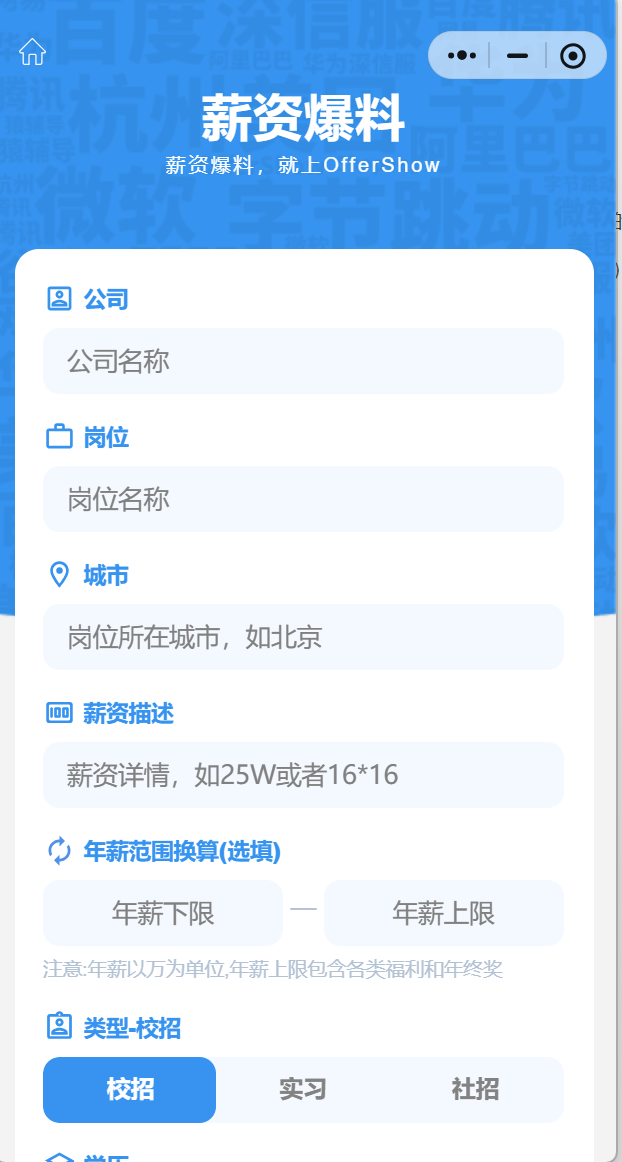
\includegraphics[width=\linewidth]{image-20260427151728493.png}
        \caption{薪资爆料表单（上半部分）}
        \label{fig:salary-report1}
    \end{minipage}\hfill
    \begin{minipage}{0.30\textwidth}
        \centering
        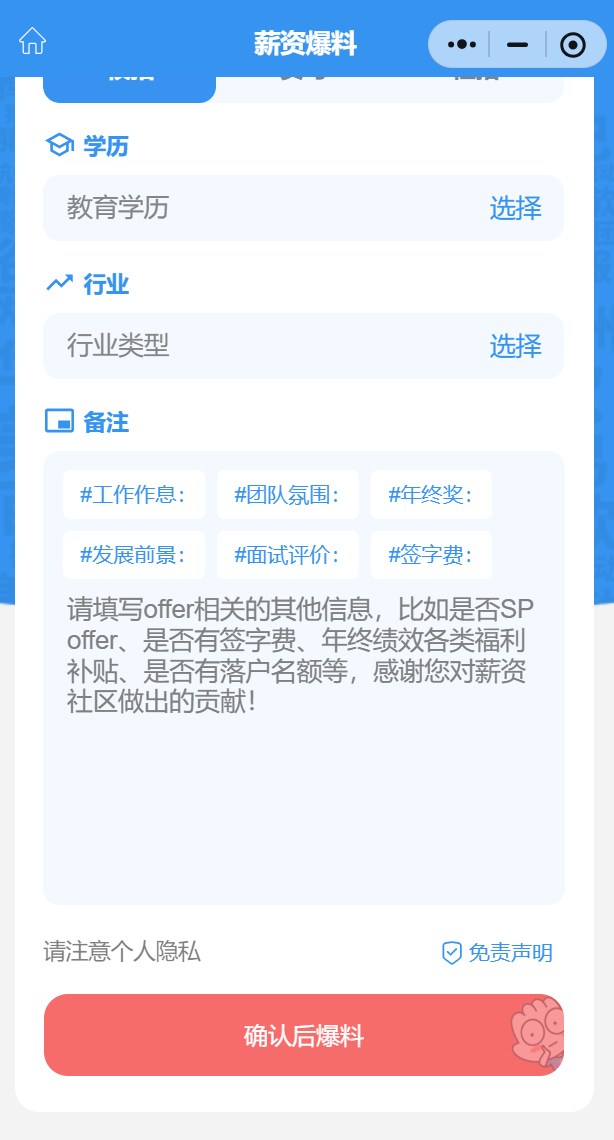
\includegraphics[width=\linewidth]{image-20260427151740530.png}
        \caption{薪资爆料表单（下半部分）}
        \label{fig:salary-report2}
    \end{minipage}
\end{figure}

\paragraph{表单字段}
\begin{itemize}[leftmargin=2em]
    \item \textbf{公司}（必填，文本，关联 \texttt{Company} 字典，自动联想）
    \item \textbf{岗位}（必填，文本，岗位名称）
    \item \textbf{城市}（必填，文本，岗位所在城市，例如"北京"）
    \item \textbf{薪资描述}（必填，文本，例如"25W"或"16*16"）
    \item \textbf{年薪范围换算}（选填，下限 / 上限两个数值，万元为单位，上限包含各类福利与年终奖）
    \item \textbf{类型}（必选 Tab：校招 / 实习 / 社招）
    \item \textbf{学历}（必选枚举：大专、本科、硕士、博士；可叠加 985/211 等标签）
    \item \textbf{行业}（必选枚举，复用招聘模块行业字典）
    \item \textbf{备注}（选填，富文本，可附 \#工作作息、\#团队氛围、\#年终奖、\#发展前景、\#面试评价、\#签字费 等标签）
    \item \textbf{免责声明}勾选；底部"确认后爆料"按钮提交。
\end{itemize}

\paragraph{业务规则}
\begin{itemize}[leftmargin=2em]
    \item 提交需登录态；同一用户对同一公司+岗位+城市组合 24 小时内不可重复提交。
    \item 系统自动生成可信度初始分（基于用户历史、信息完整度、与既有数据偏差）。
    \item 含敏感词或与历史数据严重偏离时进入人工审核队列，审核通过后入榜。
    \item 提交人个人信息匿名展示，仅显示昵称首字符或随机化标识。
\end{itemize}

\subsection{薪资最新动态（Feed）}
对应"薪资"主页 Tab，参考图~\ref{fig:salary-feed}。
\begin{figure}[H]
    \centering
    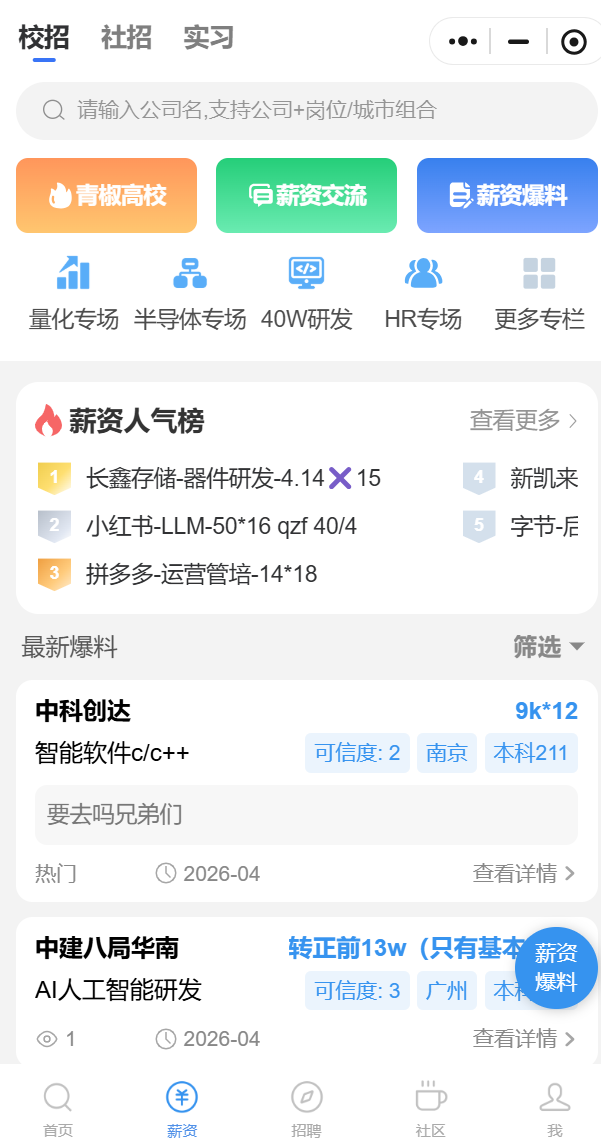
\includegraphics[width=0.30\textwidth]{image-20260427151859771.png}
    \caption{薪资最新动态主页}
    \label{fig:salary-feed}
\end{figure}

\paragraph{功能点}
\begin{itemize}[leftmargin=2em]
    \item 顶部 Tab：校招、社招、实习；切换后重新拉取列表。
    \item 顶部搜索框："请输入公司名，支持公司+岗位/城市组合"，支持组合检索（详见 \S\ref{sec:retrieval}）。
    \item 入口卡片：青椒高校、薪资交流（社群）、薪资爆料；专栏入口：量化专场、半导体专场、40W 研发、HR 专场、更多专栏。
    \item 中部精选模块"薪资人气榜"摘要（Top 5）。
    \item 底部"最新爆料"列表项字段：公司名、岗位名、薪资金额（如 \texttt{9k*12}）、可信度、城市、学历标签、用户短评、热门标记、发布月份、查看详情。
    \item 列表支持"筛选"按钮，弹出多维筛选（行业、学历、城市、薪资区间、招聘类型）；支持下拉刷新与分页加载。
\end{itemize}

\subsection{薪资人气榜单}
对应图~\ref{fig:salary-rank}。
\begin{figure}[H]
    \centering
    
\includegraphics[width=0.30\textwidth]{image-20260427151956997.png}
    \caption{薪资人气榜单（含周榜 / 月榜）}
    \label{fig:salary-rank}
\end{figure}

\paragraph{功能点}
\begin{itemize}[leftmargin=2em]
    \item 顶部统计：累计浏览人次（如 205260）、数据来源说明。
    \item 头部置顶"热门"爆料卡片。
    \item 榜单 Tab：周榜、月榜；按热度（浏览 + 点赞 + 评论加权）排序，前 N 条。
    \item 榜单条目字段：排名、公司名、岗位、薪资金额（\texttt{4.14×15} 格式）、可信度、城市、学历、热度数（火苗图标）、月份、查看详情。
    \item 支持点击进入对应薪资爆料详情页（评论 / 点赞 / 举报）。
\end{itemize}

\subsection{校招薪资查询}
对应图~\ref{fig:salary-campus1} 与图~\ref{fig:salary-campus2}。

\begin{figure}[H]
    \centering
    \begin{minipage}{0.28\textwidth}
        \centering
        
\includegraphics[width=\linewidth]{image-20260427152041153.png}
        \caption{校招薪资查询首页}
        \label{fig:salary-campus1}
    \end{minipage}\hfill
    \begin{minipage}{0.28\textwidth}
        \centering
        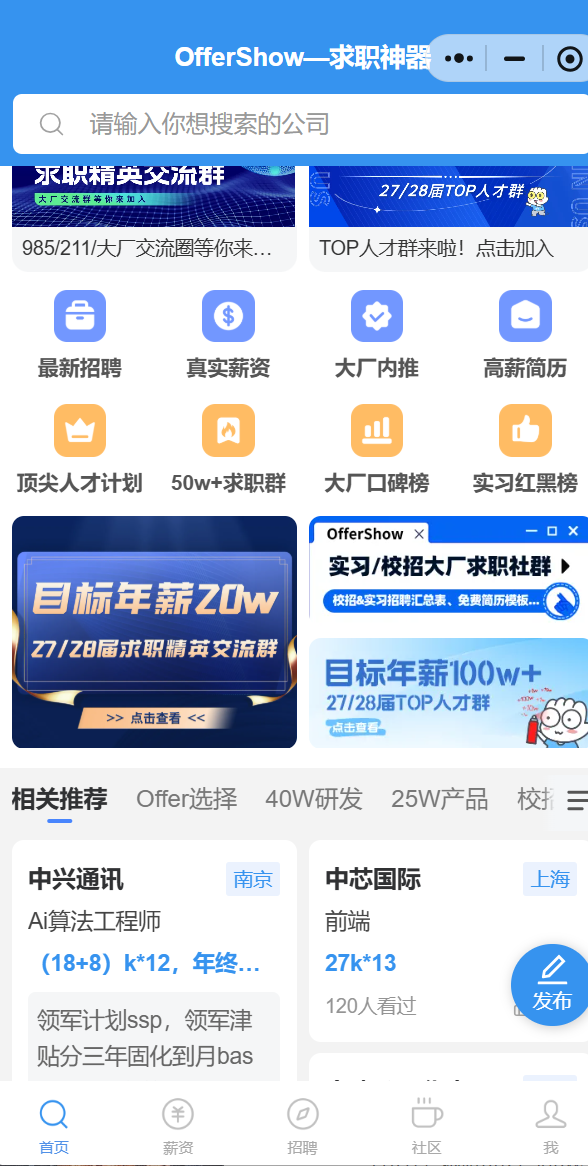
\includegraphics[width=\linewidth]{image-20260427152051535.png}
        \caption{校招薪资专栏与列表}
        \label{fig:salary-campus2}
    \end{minipage}
\end{figure}

\paragraph{功能点}
\begin{itemize}[leftmargin=2em]
    \item 顶部搜索框："查公司"，支持公司 + 岗位 / 城市组合检索；并提供"出价指南"等运营 Banner。
    \item 推荐 Banner：985/211 党专场、爆料合集、京职场真交流、Meta-Summer 2026 等。
    \item 九宫格入口：最新爆料、985 211、薪资人才计划、外企 / 大厂入门、量化专场等专栏入口。
    \item 专栏卡片：例如"目标年薪 20W"、"目标年薪 100W+"；点击进入对应薪资聚合页。
    \item "相关爆料"列表：默认按"校招"维度展示最新薪资爆料。
    \item 数据范围：仅 \texttt{recruitment\_type = 校招} 的薪资记录。
\end{itemize}

\subsection{社招薪资查询}
对应图~\ref{fig:salary-social}。

\begin{figure}[H]
    \centering
    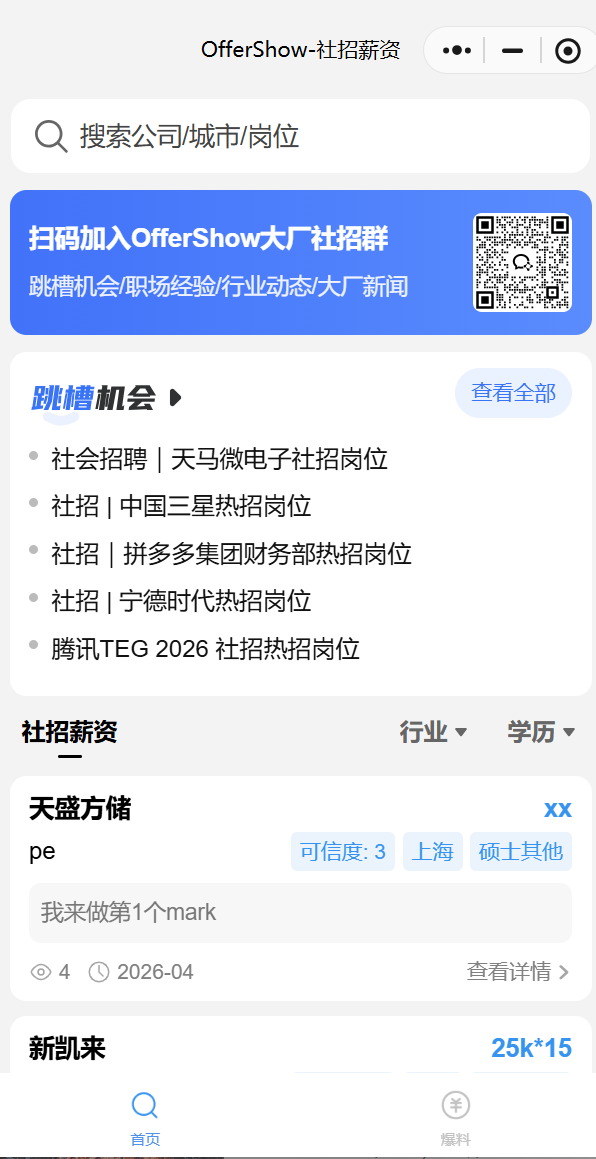
\includegraphics[width=0.30\textwidth]{image-20260427152135358.png}
    \caption{OfferShow 社招薪资查询页}
    \label{fig:salary-social}
\end{figure}

\paragraph{功能点}
\begin{itemize}[leftmargin=2em]
    \item 顶部搜索框："搜索公司 / 城市 / 岗位"。
    \item 顶部 Banner：扫码加入 OfferShow 大厂社招群（跳槽机会 / 职场经验 / 行业动态 / 大厂新闻）。
    \item "跳槽机会"专栏：列出当下社招热招岗位条目，例如"社招 | 中国三星热招岗位"、"腾讯 TEG 2026 社招热招岗位"等；右侧"查看全部"。
    \item "社招薪资"列表：含"行业"、"学历"两个下拉筛选；条目字段：公司名、岗位、薪资金额（如 \texttt{25k*15}）、可信度、城市、学历、用户短评、浏览数、月份、查看详情。
    \item 数据范围：仅 \texttt{recruitment\_type = 社招} 的薪资记录。
\end{itemize}

\subsection{薪资详情页}
所有列表点击"查看详情"后进入。需展示：公司名、岗位、城市、薪资描述、年薪折算、招聘类型、学历、行业、备注、可信度、提交时间；并支持点赞、评论、收藏、举报操作。评论遵循实名（OpenID）+ 敏感词过滤，刷量与异常点赞将被风控。

\section{数据对象}
为后续系统详细设计奠定基础，本节列出本模块涉及的主要资源对象。
\begin{longtable}{p{3.2cm}p{11cm}}
\toprule
\textbf{对象} & \textbf{关键字段}\\
\midrule
\endhead
Company（公司） & id、name、logo\_url、industry、scale、intro、country\_list\\
JobPosting（招聘信息） & id、company\_id、title、batch（招聘批次）、cities[]、industry、recruitment\_type、deliver\_start、deliver\_end、graduation\_range、apply\_url、internal\_code、benefits[]、views、interest\_count、status\\
Position（招聘岗位） & id、posting\_id、name、description\\
Industry / City / Batch & 字典表，由管理员维护\\
Subscription（早报订阅） & id、user\_id、subscribe\_date、status\\
Course（求职好课） & id、title、cover、category、price、url\\
Column（求职专栏） & id、name、description、posting\_ids[]\\
Review（实习点评） & id、company\_id、user\_id、score、content、created\_at\\
EliteProgram（顶尖人才计划） & id、company\_id、name、salary\_range、description、apply\_url\\
SalaryReport（薪资爆料） & id、company\_id、position、city、salary\_desc、annual\_min、annual\_max、recruitment\_type（校招/实习/社招）、education、industry、tags[]、remark、credibility、views、likes、status、author\_id、created\_at\\
SalaryColumn（薪资专栏） & id、name（量化专场 / 半导体专场 / 40W 研发 / HR 专场 / 985\_211 / 目标年薪 20W / 目标年薪 100W 等）、filter\_rule、cover\\
SalaryComment（薪资爆料评论） & id、report\_id、user\_id、content、likes、created\_at\\
User（用户） & id、openid、role、is\_member、is\_blocked\\
\bottomrule
\end{longtable}

\section{对外功能与作业要求映射}
本模块在系统实现中需满足课程作业要求中规定的能力，分项映射如下。

\subsection{标准方法}
针对核心资源 \texttt{JobPosting}、\texttt{SalaryReport}（亦适用于 \texttt{Company}、\texttt{Review}、\texttt{SalaryComment} 等）需实现：
\begin{itemize}[leftmargin=2em]
    \item \textbf{Get}：根据 id 获取一条招聘信息 / 薪资爆料详情。
    \item \textbf{List}：分页 + 多条件筛选（行业、城市、招聘类型、学历、薪资区间、批次、关键字）列出资源。
    \item \textbf{Create}：HR / 管理员创建招聘；登录用户提交一条薪资爆料。
    \item \textbf{Update}：作者 / 管理员部分字段更新（PATCH），如修改备注、补充福利。
    \item \textbf{Replace}：管理员整体替换（PUT），常用于审核后的字段标准化。
    \item \textbf{Delete}：作者 / 管理员删除或下架招聘信息 / 薪资爆料。
\end{itemize}

\subsection{部分检索（关键字搜索）}\label{sec:retrieval}
\begin{itemize}[leftmargin=2em]
    \item 招聘首页搜索框：模糊匹配公司名、招聘标题、岗位名。例如输入"字节跳动"返回所有名称包含"字节跳动"的招聘。
    \item 实习点评榜搜索：模糊匹配 \texttt{Company.name}。
    \item 薪资页面搜索框：支持"公司"、"公司+岗位"、"公司+城市"、"公司+岗位+城市"组合检索；搜索结果按招聘类型 Tab 分桶。
    \item 社招薪资搜索：模糊匹配公司、城市、岗位三个字段中的任一。
    \item 排序方式：相关度、最新、热度（浏览 + 点赞加权）。
\end{itemize}

\subsection{批处理}
\begin{itemize}[leftmargin=2em]
    \item HR 用户可通过 Excel/CSV 批量上传招聘信息（BatchCreate JobPostings）。
    \item 管理员可批量下架、批量审核（BatchUpdate / BatchDelete）招聘信息与薪资爆料。
    \item 求职专栏 / 内推合集 / 薪资专栏支持批量将多条记录加入或移出。
    \item 数据迁移 / 运营导入场景支持批量导入历史薪资数据（BatchCreate SalaryReports，需打"运营导入"标记）。
\end{itemize}

\subsection{分页}
\begin{itemize}[leftmargin=2em]
    \item 所有 List 类接口需支持基于 \texttt{page\_size} + \texttt{page\_token}（或 \texttt{page}）的分页。
    \item 默认每页 20 条，最大 50 条；返回 \texttt{next\_page\_token} 用于下一页拉取。
    \item 应用于：招聘信息列表、求职早报当日 24h 新招、社招集合、内推集合、点评列表、薪资爆料 Feed、薪资人气榜、校招/社招薪资查询、薪资爆料评论列表等。
\end{itemize}

\subsection{权限控制}
\begin{itemize}[leftmargin=2em]
    \item 基于角色的访问控制（RBAC）：游客 / 普通用户 / 会员 / HR / 管理员。
    \item 防作弊：对短时间内高频上传/打分的用户进行限流并打标，作弊用户的写操作被拒绝；可由管理员封禁。
    \item 反爬：对未登录或异常 UA / 高频 IP 的 List 接口加风控（限流、滑块、token 校验）。
    \item 资源所有权：HR 仅能操作其所属公司的招聘信息；普通用户仅能修改/删除自己创建的点评、薪资爆料与评论。
    \item 会员特权：开通会员后可查看"提前看"招聘列表、领取专属内推码、查看完整薪资详情（非会员对部分热门爆料的金额做模糊化展示）。
    \item 薪资爆料的反作弊与反爬：金额异常（偏离同公司同岗位中位数过远）、短时高频提交、相同 IP/设备多账号提交，均触发风控降权或人工审核。
\end{itemize}

\section{非功能性需求}
\begin{itemize}[leftmargin=2em]
    \item \textbf{性能}：首页列表 P95 响应时间 \textless~500ms；搜索 P95 \textless~800ms。
    \item \textbf{可用性}：核心列表与详情接口 SLA 99.9\%。
    \item \textbf{可扩展性}：行业、城市、招聘批次均通过字典服务维护，可在后台动态扩充。
    \item \textbf{安全}：所有写操作需登录态 + CSRF/Token 校验；敏感字段（投递链接、内推码）按权限脱敏。
    \item \textbf{合规}：用户点评需经过敏感词过滤；招聘信息发布须通过审核。
\end{itemize}

\section{参考来源}
\begin{itemize}[leftmargin=2em]
    \item Offer Show 微信小程序"找名企 $\rightarrow$ 名企实习校招"与"查薪资"。
    \item 课程作业要求。
\end{itemize}

\end{document}
